\documentclass{beamer}
\usetheme{Marburg}
\usepackage{tikz}
\usepackage{soul}
\usepackage{tabularx}
\usepackage{paralist}
%\usepackage{listings}
\usepackage{color} % for coloured text
%\usepackage{listings} % for code listings
\usepackage{amsmath} % for math!
\usepackage{graphicx} % for pictures...
%\usepackage{caption} % for margin figures
\usepackage{hyperref} % links
\usepackage{natbib}
%\usepackage{booktabs}
%\usepackage{gensymb}
\usepackage{comment}
\usepackage[algo2e]{algorithm2e}
%\usepackage{algpseudocode}
\newcommand{\bdp}{\mathbf{\Delta p}}
\newcommand{\bSig}{\mathbf{\Sigma}}
\newcommand{\rT}{\mathrm{T}}
\newcommand{\bb}{\mathbf{b}}
\renewcommand{\bf}{\mathbf{f}}
\newcommand{\bp}{\mathbf{p}}
\newcommand{\br}{\mathbf{r}}
\newcommand{\bs}{\mathbf{s}}
\newcommand{\bt}{\mathbf{t}}
\newcommand{\bx}{\mathbf{x}}
\newcommand{\by}{\mathbf{y}}

\newcommand{\bA}{\mathbf{A}}
\newcommand{\bF}{\mathbf{F}}
\newcommand{\bI}{\mathbf{I}}
\newcommand{\bJ}{\mathbf{J}}
\newcommand{\bR}{\mathbf{R}}
\newcommand{\bS}{\mathbf{S}}
\newcommand{\bT}{\mathbf{T}}
\newcommand{\bX}{\mathbf{X}}

\newcommand{\inv}[1]{#1^{-1}}
\newcommand{\abs}[1]{\left\lvert #1\right\rvert}
\newcommand{\norm}[1]{\left\lvert\left\lvert #1\right\rvert\right\rvert}
\newcommand{\qmark}[1]{\mbox{}\hfill\textbf{[#1]}}
\newcommand{\argmin}{\operatorname*{arg\,min}}
\newcommand{\argmax}{\operatorname*{arg\,max}}
\newcommand{\var}{\operatorname*{var}}
\newcommand{\diag}{\operatorname*{diag}}
\newcommand{\tr}{\operatorname*{Tr}}
\newcommand{\dcos}{d_\mathrm{cos}}
\newcommand{\deuc}{d_\mathrm{euc}}
 % New commands
%\usepackage{framed}
%\lstset{
%  language=matlab,
%  basicstyle=\ttfamily,
%  keywordstyle=\ttfamily
%}


\title{06 22313 Computational Tools for Modelling and Analysis}
\subtitle{Identifying Groups in Data}
\author{Dr Iain Styles (I.B.Styles@bham.ac.uk)}
\institute{School of Computer Science, University of Birmingham}
\date{November 2 2015}

\begin{document}

\begin{frame}
  \titlepage
\end{frame}

\begin{frame}{Outline}
  \tableofcontents
\end{frame}

\section{Introduction}

\begin{frame}{Introduction}

  \begin{itemize}
  \item Fitting lines to data works well if a line is a good description of your data!
  \item There are many cases where this is not the case, for example when the data is composed of groups of points.
  \item We would want to identify what these groups were rather than just trying to fit some line to them.
  \end{itemize}
\begin{center}
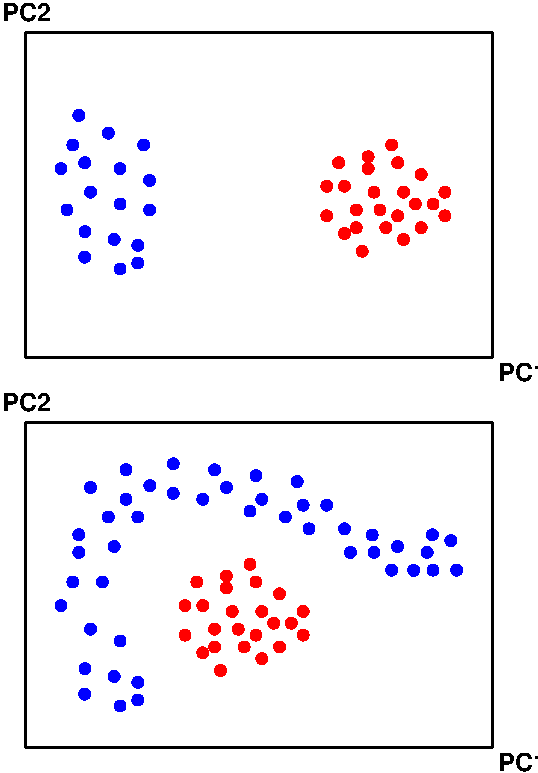
\includegraphics[width=\textwidth]{simpleclusters}
\end{center}
\end{frame}

\begin{frame}{Why might data be clustered?}
  \begin{center}
    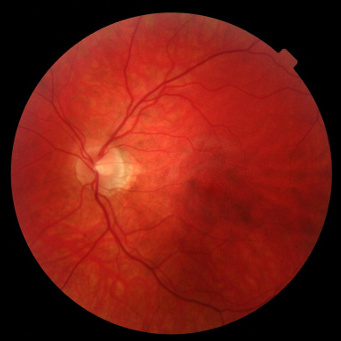
\includegraphics[width=0.38\textwidth]{rgbeye}
    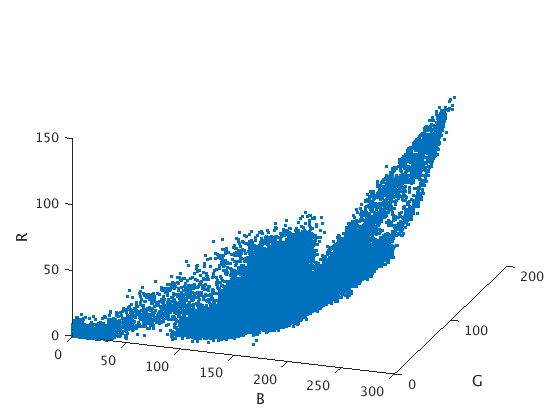
\includegraphics[width=0.58\textwidth]{rgbeyecluster}
  \end{center}
\end{frame}

\begin{frame}{General Approaches to Clustering}
  \begin{itemize}
    \item Hundreds of clustering algorithms,
    \item Many assume something about the data, eg clusters are normally distributed.
    \item Most are based on grouping points that are ``similar''
    \item Outcome is sets (groups) of points that by some measure ``belong together''.
    \item Main approaches are:
      \begin{itemize}
        \item Bottom-up
        \item Top-down
      \end{itemize}
  \end{itemize}

\end{frame}

\section{Measures of Similarity}
\begin{frame}{Measures of Similarity}
  \begin{itemize}
    \item The key issue in clustering is how to measure ``similarity''
    \item Two important issues:
      \begin{itemize}
        \item What is the appropriate measure of similarity of two data points?
        \item How do you measure the similarity of groups of points?
      \end{itemize}
  \end{itemize}
\end{frame}


\begin{frame}{Euclidean Distance}
  \begin{itemize}
    \item Intuition: similarity $\leftrightarrow$ ``closeness''
    \item So measure the distance between points
    \item Most common is \textbf{Euclidean distance}.
      \begin{itemize}
        \item Given data points $\bx^{(1)}$ and $\bx^{(2)}$:
      \end{itemize}
  \end{itemize}

      \begin{equation*}
        \deuc(\bx^{(1)},\bx^{(2)}) = \sqrt{\sum_{i=1}^M \left[x_i^{(1)} - x_i^{(2)}\right]^2}
      \end{equation*}

  \begin{minipage}{0.4\textwidth}
      \begin{center}
        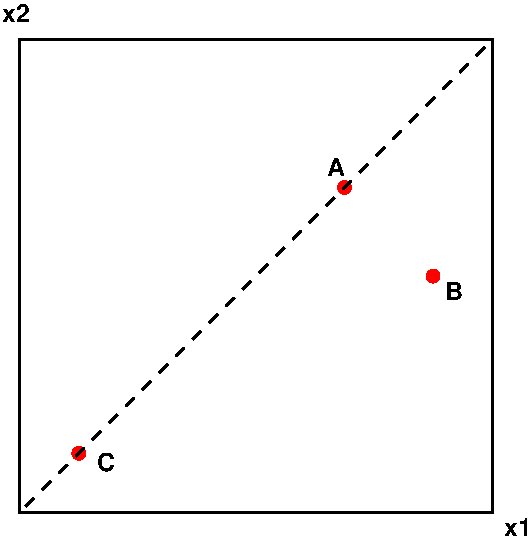
\includegraphics[width=\textwidth]{distances}
      \end{center}
  \end{minipage}
  \begin{minipage}{0.55\textwidth}
      Which points are closest/most similar?
  \end{minipage}
\end{frame}

\begin{frame}{Euclidean Distance}
  \begin{itemize}
    \item A and B are closest in the Euclidean sense
    \item But A and C are also similar in a different sense: direction
    \item A and C are in the ``direction'' from the original but are scaled
      \begin{itemize}
        \item In a colour space, A and C are the same hue but A is brighter.
        \item B is similar brightness as A, but a different hue.
      \end{itemize}
    \item This type of similarity is captured by a different similarity (distance) measure
  \end{itemize}
\end{frame}

\begin{frame}{Cosine Distance}
  \begin{equation*}
    \dcos(\bx^{(1)},\bx^{(2)}) = \cos^{-1}\left(\frac{\bx^{(1)}\cdot\bx^{(2)}}{\norm{\bx^{(1)}}_2\norm{\bx^{(2)}}_2}\right)
  \end{equation*}

  \begin{itemize}
    \item Cosine distance between A and C is zero
      \begin{itemize}
        \item Both at the same angle relative to the origin
        \item Captured by this metric
      \end{itemize}
    \item Choice of similarity measure is highly dependent on the nature of your dataset and on what properties you want to capture in your clusters
    \item Not the only choices: also correlation, Manhattan and Mahalanobis distances.
  \end{itemize}
\end{frame}

\section{Normalisation}
\begin{frame}{Normalisation}
  \begin{itemize}
    \item The same considerations also lead us to consider ``normalising''  each item of data
    \item For example, we could normalise the points all have the same length:
      \begin{equation*}
        \sqrt{\sum_{i=1}^nx_i^2}=\sqrt{\bx^\rT\bx}=1 \quad\mapsto\quad \bx\gets\frac{\bx}{\sqrt{\bx^\rT\bx}}
      \end{equation*}.
      \item Removes global ``intensity'' differences from the data.
      \item Draws all points radially onto the unit circle.
      \item A and C now co-incident
      \item Whether you should do this depends on what properties you wish to cluster against.
  \end{itemize}

\end{frame}

\section{Linkage}

\begin{frame}{Linkage}
  \begin{itemize}
    \item How do we measure similarities between groups?
    \begin{itemize}
      \item Single Linkage\\
        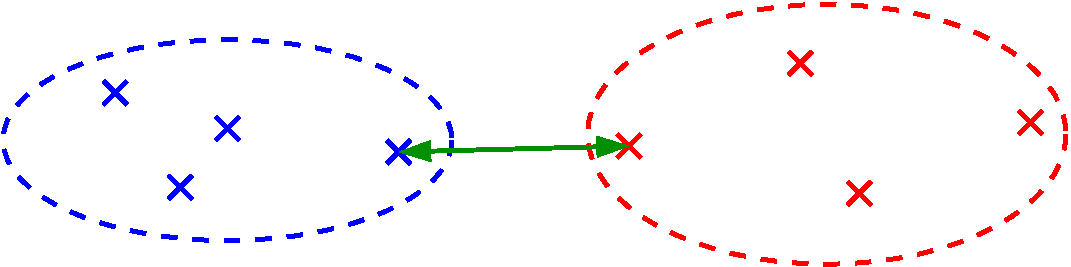
\includegraphics[width=0.7\textwidth]{singlelinkage}
      \item Average Linkage\\
        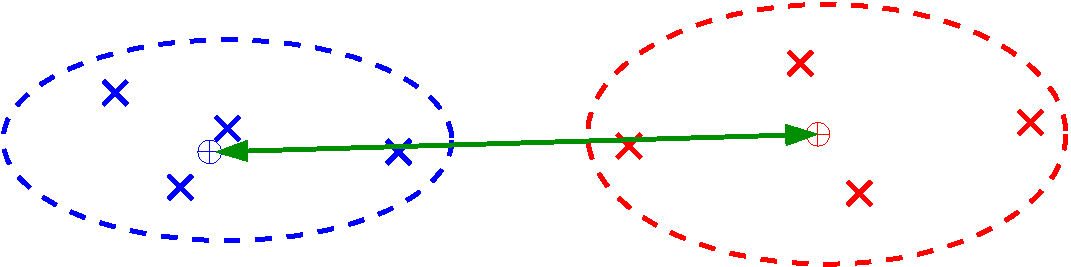
\includegraphics[width=0.7\textwidth]{averagelinkage}
      \item Complete Linkage\\
        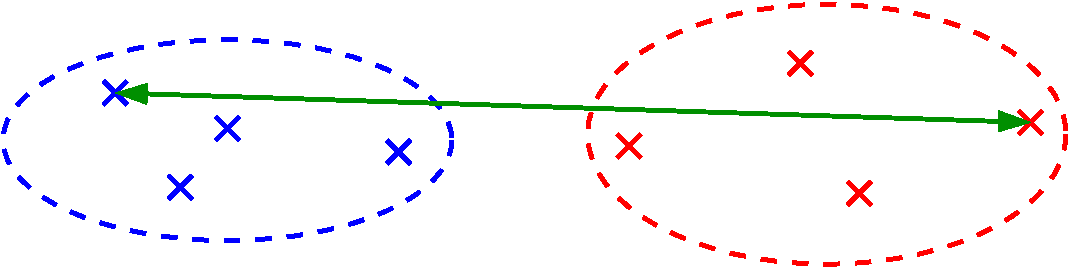
\includegraphics[width=0.7\textwidth]{completelinkage}
    \end{itemize}
  \end{itemize}
\end{frame}



\section{The k-means Algorithm}
\begin{frame}{The $k$-means Algorithm}
  \begin{itemize}
    \item Perhape the most commonly used clustering technique
    \item Partitions $N$ data points into $k<N$ clusters
    \item Each data point belongs to the ``nearest'' cluster (nearest mean)
    \item Cluster boundaries are straight lines bisect those connecting the means
    \item Regions define by these lines define the clusters
    \item We will use Euclidean distance here, but other distance measures can be used.
    \begin{center}
      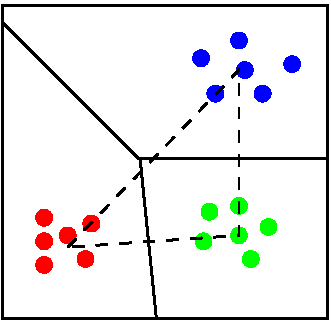
\includegraphics[width=0.4\textwidth]{kmeans-part}
    \end{center}
  \end{itemize}
\end{frame}

\begin{frame}{The $k$-means Algorithm}
  \begin{itemize}
    \item Number of clusters $k$ is specified by the ``user''. 
    \begin{itemize}
      \item[1)] First, randommly assign every data point to one of the clusters.
      \item[2)] Compute the mean position (in the data space) of each cluster
      \item[3)] For each data point, calculate distance to mean of each cluster
      \item[4)] Re-assign points to their nearest cluster.
      \item[5)] Return to step 2 and repeat until the clusters are not changing.
    \end{itemize}
  \end{itemize}
\end{frame}

\begin{frame}{Notes about $k$-means}
  There are a few points to note:
  \begin{itemize}
    \item Initial random seeding $\rightarrow$ repeats needed
    \item Have to ``guess'' the number of clusters.
    \begin{itemize}
      \item Too many, and you will split what should be a single cluster.
      \item Too few, and you will combine clusters that should be separate, or splitting clusters and merge with others.
    \end{itemize}
    \item This is a computationally ``hard'' algorithm (in the jargon, it is NP-hard).
      \begin{itemize}
        \item The number of distance calculations increases rapidly with the number of clusters and the number of data points so it can be very costly for large datasets.
      \end{itemize}
    \item Works with all distance measures, although the ``shape'' of the clusters will be less intuitive.
    \item Linkage strategies are not required as the only distances computed are between the points and the means.
  \end{itemize}
\end{frame}

\begin{frame}{The $k$-means Algorithm}
    \begin{center}
      \only<1>{
        Initial data points

        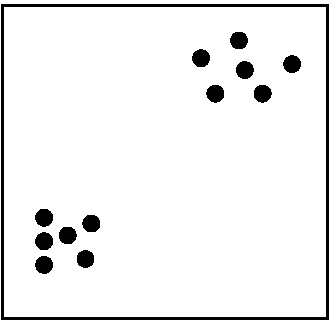
\includegraphics[height=0.6\textwidth]{kmeans1}
      }
      \only<2>{
        Randomly assign points to groups

        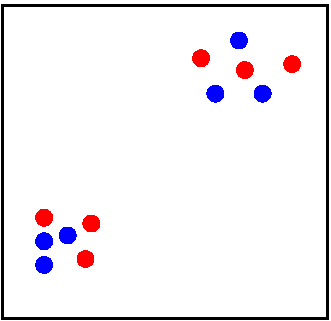
\includegraphics[height=0.6\textwidth]{kmeans2}
      }
      \only<3>{
        Compute group average

        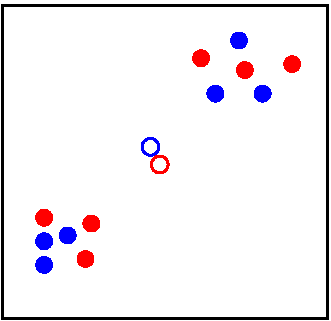
\includegraphics[height=0.6\textwidth]{kmeans2av}
      }
      \only<4>{
        Re-assign points to groups

        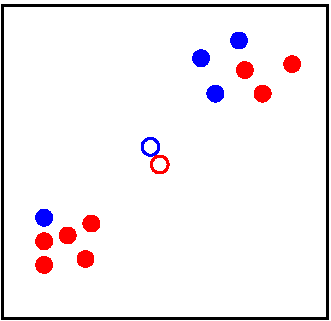
\includegraphics[height=0.6\textwidth]{kmeans3}
      }
      \only<5>{
        Re-compute group averages

        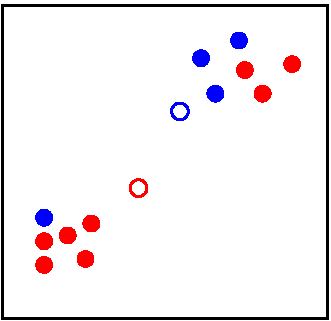
\includegraphics[height=0.6\textwidth]{kmeans3av}
      }
      \only<6>{
        Re-assign points to groups

        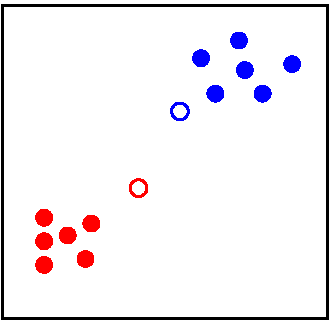
\includegraphics[height=0.6\textwidth]{kmeans4}
      }
      \only<7>{
        Re-compute group averages

        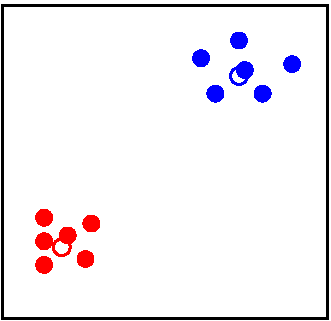
\includegraphics[height=0.6\textwidth]{kmeans4av}
      }
    \end{center}
\end{frame}

\begin{frame}{The k-means Algorithm}
  \scalebox{0.4}{
    \begin{minipage}{\linewidth}
      \begin{algorithm2e}[H]
        \SetLine

  \SetKwComment{com}{\% }{}
  \KwData{Data points $Data[N]$; Number of clusters $K$}
  \KwResult{$\bp,e(\bp)$, parameters that minimmise the least squares error, the error.}

  \com{Randomly assign each point to a cluster}
  \For{$i\gets 1$ \KwTo $N$}{
    $ClusterIndex[i]\gets randint(1,K)$
  }
  \com{Calculate the mean of each cluster}
  \For{$i\gets 1$ \KwTo $K$}{
    $ClusterMean[i] \gets mean(Data[Cluster[i]])$
  }

  \com{Iterate until clusters are stable}
  $Converged\gets False$\;
  \While{$Converged==False$}{

      \com{Compute distance from every point to each cluster mean}
      \For{$i\gets 1$ \KwTo $K$}{
        \For{$j\gets 1$ \KwTo $N$}{
          $dist[i][j] \gets distance(ClusterMean[i],Data[j])$
        }
      }

      \com{Find the nearest mean for each data point}
      \For{$i\gets 1$ \KwTo $N$}{
        \For{$j\gets 1$ \KwTo $K$}{
          $NewClusterIndex[i] = nearest(Data[i],ClusterMean[j])$
        }
      }

      \com{Generate new clusters}
      \For{$j\gets 1$ \KwTo $K$}{
        $ClusterMean[i] \gets mean(Data[NewClusterIndex==i])$
      }

      \com{Check to see if cluster membership has changed}
      $Converged\gets True$

      \If{NewClusterIndex != ClusterIndex}{
          $Converged \gets False$
      }

      \com{Replace old clusters with new ones}
      $ClusterIndex \gets NewClusterIndex$
      $ClusterMean \gets NewClusterMean$
  }
  \caption{The $k$-Means Algorithm.}
  \label{alg:kmeans}
      \end{algorithm2e}
    \end{minipage}
  }
\end{frame}
%
\section{Agglomerative Clustering}
\begin{frame}{Agglomerative Clustering}
  \begin{itemize}
    \item $k$-means is a top-down algorithm.
    \item Clusters are ``flat'' with no structure.
    \item Change $k$ $\rightarrow$ must recluster.
    \item Strict convex partitioning not appropriate for many types of data.
    \item Hierarchical clustering is an alternative ``bottom-up'' strategy
    \item Sequentially pair closest point together.
  \end{itemize}
\end{frame}

\begin{frame}{Agglomerative Clustering}
  \begin{itemize}
    \item[1)] Compute distances between all pair of data points
    \item[2)] Find the closest pair
    \item[3)] Remove this pair from the dataset and replace it with the grouped pair.
    \item[4)] Recalculate distances between all points and the new group using a linkage strategy.
    \item[5)] Go to 2) and continue grouping until all points are grouped
  \end{itemize}
\end{frame}

\begin{frame}{Agglomerative Clustering}
  \begin{center}
    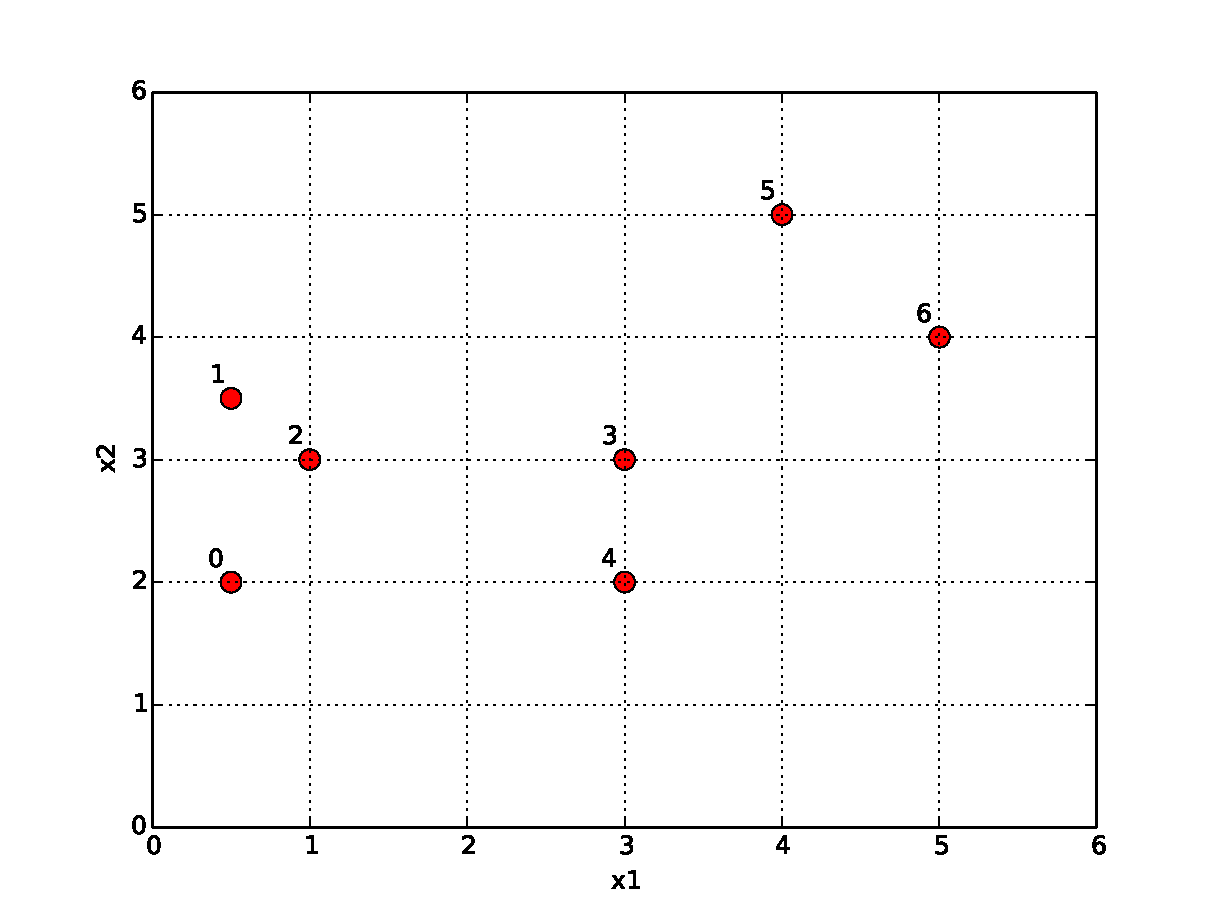
\includegraphics[width=0.6\textwidth]{hierpts}

    \begin{tabular}{lcl}
      List of points & &0,1,2,3,4,5,6\\ \pause
      Group 1 with 2 &$\mapsto$ &0,3,4,5,6,(1,2)\\\pause
      Group 3 with 4&$\mapsto$ &0,5,6,(1,2),(3,4)\\\pause
      Group 0 with (1,2)&$\mapsto$ &5,6,(3,4),(0,(1,2))\\\pause
      Group 5 with 6&$\mapsto$&(3,4),(0,(1,2)),(5,6)\\\pause
      Group (3,4) with (0,(1,2)) &$\mapsto$&(5,6),((3,4),(0,(1,2)))\\\pause
      Group (5,6) with ((3,4),(0,(1,2)))&$\mapsto$&((5,6),((3,4),(0,(1,2))))
    \end{tabular}
  \end{center}
\end{frame}

\begin{frame}{Agglomerative Clustering}
  \begin{itemize}
    \item Represent as a \textbf{dendrogram} where the height of each ``junction'' in the dendrogram represents the distance 
      \begin{itemize}
        \item Eg. $(3,4)$ join at height 1.
      \end{itemize}
  \end{itemize}

      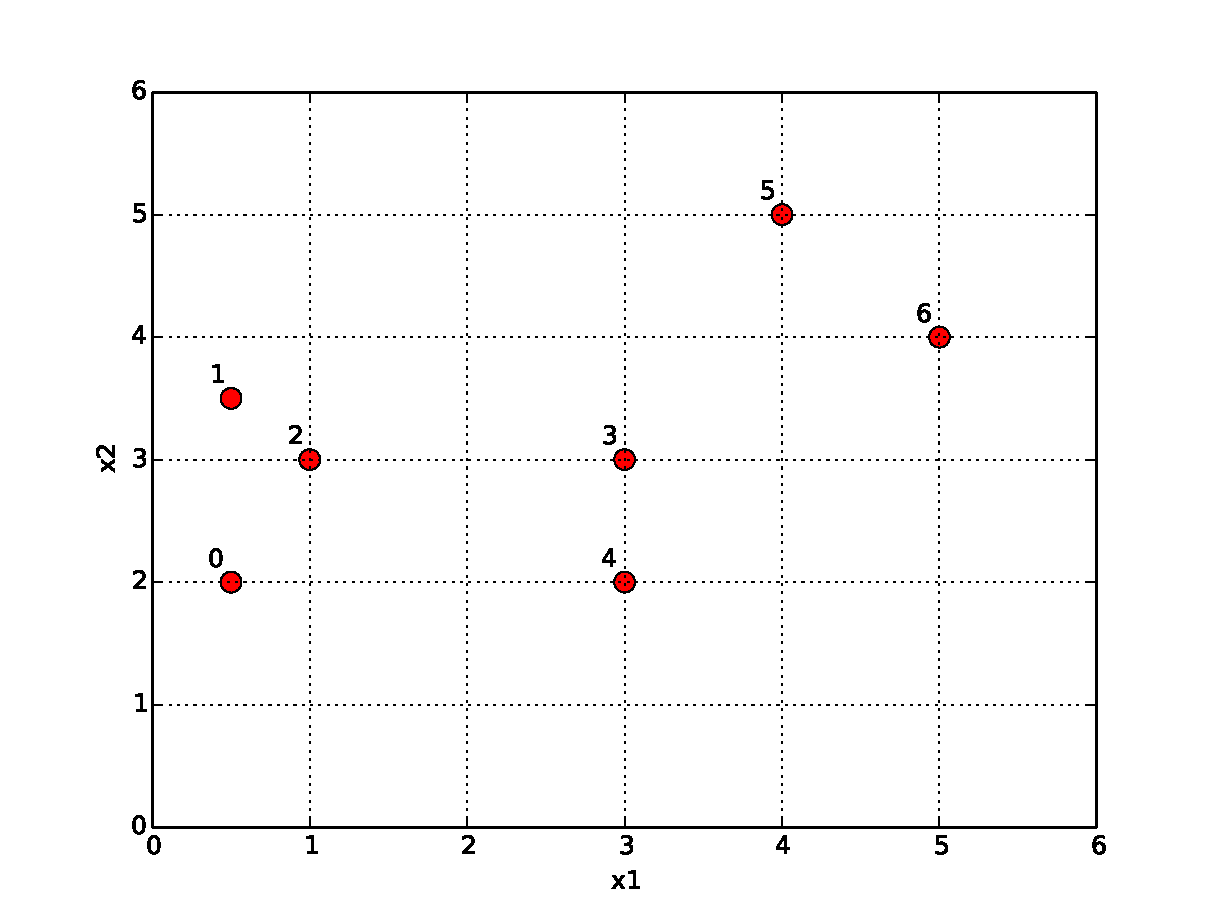
\includegraphics[width=0.5\textwidth]{hierpts}
      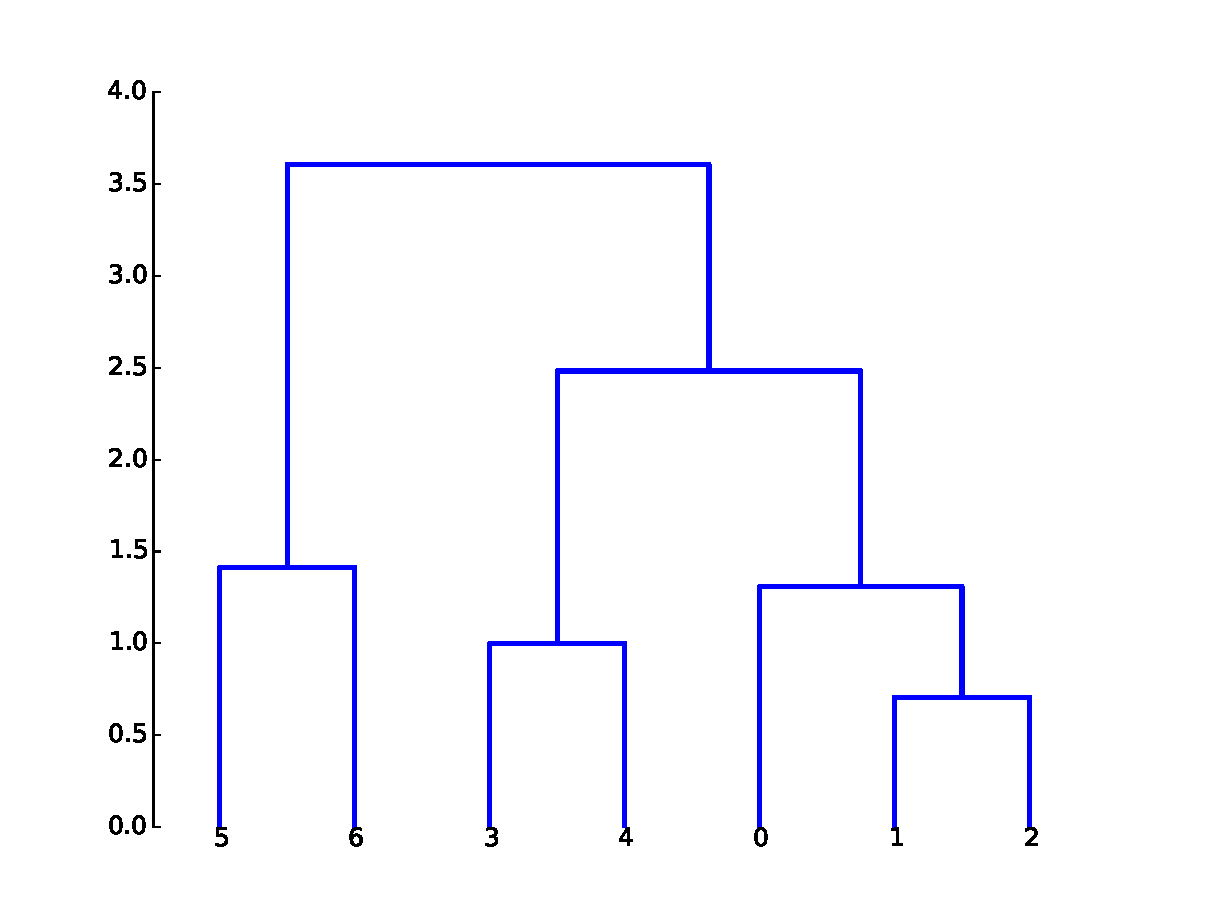
\includegraphics[width=0.5\textwidth]{dendro}
\end{frame}

\begin{frame}{Agglomerative Clustering}
  \begin{itemize}
    \item Generates all numbers of clusters. 
      \begin{itemize}
        \item Cut horizontally across the dendrogram.
      \end{itemize}
    \item But many computations
      \begin{itemize}
        \item $k$-means: $N$ points, $K$ cluster $\rightarrow N\times K$ distances
        \item Hierarchical: ``choose 2 from N'' $=\frac{n!}{2\,(n-2)!}$ calculations just for first pairing.
      \end{itemize}
    \item $k$-means faster if you know how many clusters, but if you don't will have to run multiple times and for multiple repeats.
    \item They will NOT normally give identical results: choice depends on nature of data.
  \end{itemize}
\end{frame}

\section{Other Clustering Methods}
\begin{frame}{Other Clustering Methods}
  \begin{itemize}
    \item Two of many available clustering techniques, but common choices.
    \item Still many free choices:
    \begin{itemize}
      \item How many clusters? Which distance metric? What linkage method?
    \end{itemize}
    \item Optimal combination often trial-and-error, but some ``internal'' validation measures can be used.
    \item Should understand the assumptiona and types of cluster you can get before choosing.
    \item Many clustering tools are available.
    \begin{itemize}
      \item Matlab Statistics Toolbox includes many
      \item ELKI (Environment for Developing KDD-Applications Supported by Index-Structures) from \url{http://elki.dbs.ifi.lmu.de/} includes many advanced techniques e.g. DBSCAN\citep{ester1996density}.
    \end{itemize}
  \end{itemize}
  {\tiny
    \bibliographystyle{alpha}
    \bibliography{clustering}
  }
\end{frame}

\end{document}
